\documentclass[11pt]{article}
% \def\hidesolutions{}
%%%%%%%%%%% SET MARGINS
\setlength{\textheight}{20cm}
\setlength{\topmargin}{-0.5cm}
\setlength{\oddsidemargin}{+0cm}
\setlength{\textwidth}{16.3cm}
%\setlength{\parskip}{6pt}
\setlength{\parindent}{0pt}

%%%%%%%%%%% PACKAGES
\usepackage{amsmath}
\usepackage{amssymb}
\usepackage{amsfonts}
%\usepackage{a4wide}
\usepackage{graphicx}
\usepackage{color}
\usepackage[normalem]{ulem}
\usepackage{enumitem}
\usepackage{capt-of}
\usepackage{float}
\usepackage{amsmath}
\usepackage{listings}
\definecolor{mygreen}{RGB}{28,172,0} % color values Red, Green, Blue
\definecolor{mylilas}{RGB}{170,55,241}
\usepackage{empheq}
\usepackage[ruled]{algorithm2e}
\usepackage{mathrsfs}
\usepackage{datetime}
\usepackage{subcaption}

% TODO: combine the two package lists and reduce redundancies 
\usepackage{mathtools}
\usepackage{nicefrac}
\usepackage{hyperref}
\usepackage{url}
\usepackage{amsmath,amssymb,amsfonts}
\usepackage{a4wide}
\usepackage{graphicx}
\usepackage{color}
\usepackage[normalem]{ulem}
\usepackage{capt-of}
\usepackage{float}
\usepackage[ruled]{algorithm2e}
\usepackage{amsmath,amssymb,amsfonts}
\usepackage{a4wide}
\usepackage{graphicx}
\usepackage{color}
\usepackage[normalem]{ulem}
\usepackage{capt-of}
\usepackage{float}
\usepackage[ruled]{algorithm2e}
\usepackage{mathrsfs}







\newcommand{\Lc}[2]{{\color{blue} \sout{#1} } \textcolor{red}{#2}}
\newcommand{\La}[1]{\textcolor{red}{#1}}
\newcommand{\lh}{\mathscr{L}_h}
\newcommand{\cl}{\mathscr{L}}
\newcommand{\cf}{\mathscr{F}}
\newcommand{\dx}{dx}
\newcommand{\ltn}{\mathscr{l}^2}
\newcommand{\bbR}{\mathbb{R}}
\newcommand{\Rset}{\mathbb{R}}
\newcommand{\Nset}{\mathbb{N}}
\newcommand{\scL}{\mathcal{L}}
\newcommand{\xx}{\mathbf{x}}
\newcommand{\norm}[1]{\|{#1}\|}
\newcommand{\yy}{\mathbf{y}}
\newcommand{\at}[1]{\big|_{#1}}
\renewcommand{\div}{\mathrm{div}}
\newcommand{\divergence}{\mathrm{div}}
\newcommand{\cp}[1]{\textcolor{blue}{#1}}

\newcommand{\FF}{\texttt{FreeFem++ }}
\newcommand{\FFns}{\texttt{FreeFem++}}
\newcommand{\FFfull}{\texttt{FreeFem++-x11}}
\newcommand{\cmd}[1]{ \medskip \noindent \texttt{#1} \medskip}
\newcommand{\incmd}[1]{\texttt{#1}}
\newcommand{\shrinkitems}{\addtolength{\itemsep}{-0.5\baselineskip}}
\newcommand{\mtt}[1]{\mathtt{#1}}
\newcommand{\ML}{\texttt{Matlab }}

\newcommand{\bb}{\mathbf{b}}
\newcommand{\nn}{\mathbf{n}}
\newcommand{\vecA}{\vec{A}}
\newcommand{\vecB}{\vec{B}}


\newcommand{\mesh}{\mathcal{T}_h}
\newcommand{\refel}{\widehat{K}}
\newcommand{\ver}{\mathbf{a}}
\newcommand{\refver}{\widehat{\mathbf{a}}}
\newcommand{\grad}{\nabla}
\newcommand{\refgrad}{\widehat{\nabla}}
\newcommand{\refu}{\widehat{u}}
\newcommand{\refbasis}{\widehat{\varphi}}
\newcommand{\refxx}{\widehat{\xx}}
\newcommand{\refx}{\widehat{x}}
\newcommand{\refy}{\widehat{y}}
\newcommand{\refrho}{\widehat{\rho}}
\newcommand{\refh}{\widehat{h}}






% For typesetting Python code
\newcommand{\matlab}{{\sc Matlab}\xspace}
\usepackage{listings}
\lstloadlanguages{Python}
\lstloadlanguages{csh}%
\definecolor{MyDarkGreen}{rgb}{0.0,0.4,0.0}
\definecolor{purple}{rgb}{0.58,0,0.82}
\lstset{language=Python,                    % Use Python
	%frame=single,                          % Single frame around code
	basicstyle=\ttfamily\footnotesize\color{black},
	keywordstyle=[1]\color{blue}\bf,        % Python functions bold and blue
	keywordstyle=[2]\color{purple},         % Python function arguments purple
	keywordstyle=[3]\color{red}\underbar,   % User functions underlined and blue
	commentstyle=\usefont{T1}{pcr}{m}{sl}\color{MyDarkGreen}\small,
	stringstyle=\color{purple},
	showstringspaces=false,                 % Don't put marks in string spaces
	tabsize=3,                              % 5 spaces per tab
	morekeywords={xlim,ylim,var,alpha,factorial,poissrnd,normpdf,normcdf},
	morecomment=[l][\color{blue}]{...},
	breaklines=true,
	breakatwhitespace=true,
	emptylines=1,
	mathescape=true,
	xleftmargin=0ex,
	emphstyle=\bfseries\color{red}
}





%%%%%%%%%%% MACROS NAMES
\newcommand{\lecturername}{Martin Licht}
% \newcommand{\assistantnamea}{Jochen Hinz}
% \newcommand{\assistantnameb}{Ivan Bioli}
\newcommand{\semestername}{Winter Semester 2023}
\newcommand{\lecturename}{Analysis III - 202(c)}
\DeclarePairedDelimiter\floor{\lfloor}{\rfloor}

%%%%%%%%%%% HEADER
\newdateformat{yeardate}{\THEYEAR}
\newcommand{\exsheet}[3] % input is the number of the session and the day TODO What's that
{\clearpage

	\begin{center}
		{\Large \textbf{\lecturename}}\\[2ex]
		\semestername
	\end{center}

	% \vspace{2ex}
	% \lecturername

	\vspace{2ex}
	{\Large Session #1: #3\,#2, \yeardate\today}
	%\hfill
	%{\Large EPF Lausanne}

	\hrulefill
}





\usepackage{comment}

\newtheorem{exercise}{Exercise}
\newtheorem{solutionenv}{Solution}

\newboolean{hide_solution}
\ifx\hidesolutions\undefined
\newenvironment{solution}{\begin{solutionenv}}{\end{solutionenv}}
\setboolean{hide_solution}{false}
\else
\excludecomment{solution}
\setboolean{hide_solution}{true}
\fi

\newcommand{\ifnotsolution}[1]{\ifthenelse{\boolean{hide_solution}}{#1}{}}
\newcommand{\ifsolution}[1]{\ifthenelse{\boolean{hide_solution}}{}{#1}}








\allowdisplaybreaks

\begin{document}
\exsheet{14}{19}{December} % parameters are the number of the session and the day

\begin{exercise}
    Given the following functions over an interval $[0,1)$, 
    \begin{enumerate}[label=(\alph*)]
        \item $f(x) = x$
        \item $g(x) = x^2$
        \item $h(x) = e^x$
        \item $s(x) = sin(\pi x)$
    \end{enumerate}
    sketch their extension to 
    \begin{itemize}
        \item a periodic function with period $1$,
        \item an even periodic function with period $2$,
        \item an odd periodic function with period $2$.
    \end{itemize}
    State the formulas for the even and odd $2$-periodic extensions over the interval $[-1,1]$.
\end{exercise}

\begin{solution}
    We begin with these plots:
    \begin{center}
        \begin{tabular}{cc} % 2x2 matrix structure
            % Top-left plot
            \begin{tikzpicture}[scale=0.6]
                \draw[->] (-2,0)--(2,0) node[right]{$x$};
                \draw[->] (0,-3)--(0,3) node[above]{$y$};
                % Unrolled loop for f(x)=x
                \draw[domain=-2:-1,smooth,variable=\x,blue] plot({\x},{\x+2});
                \draw[domain=-1:0,smooth,variable=\x,blue] plot({\x},{\x+1});
                \draw[domain=0:1,smooth,variable=\x,blue] plot({\x},{\x});
                \draw[domain=1:2,smooth,variable=\x,blue] plot({\x},{\x-1});
                \node[blue,above right] at (0.5,0.5) {$f(x)=x$};
            \end{tikzpicture}
            &
            % Top-right plot
            \begin{tikzpicture}[scale=0.6]
                \draw[->] (-2,0)--(2,0) node[right]{$x$};
                \draw[->] (0,-3)--(0,3) node[above]{$y$};
                % Unrolled loop for g(x)=x^2
                \draw[domain=-2:-1,smooth,variable=\x,red] plot({\x},{(\x+2)*(\x+2)});
                \draw[domain=-1:0,smooth,variable=\x,red] plot({\x},{(\x+1)*(\x+1)});
                \draw[domain=0:1,smooth,variable=\x,red] plot({\x},{\x*\x});
                \draw[domain=1:2,smooth,variable=\x,red] plot({\x},{(\x-1)*(\x-1)});
                \node[red,above] at (0.5,0.5) {$g(x)=x^2$};
            \end{tikzpicture}
            \\
            % Bottom-left plot
            \begin{tikzpicture}[scale=0.6]
                \draw[->] (-2,0)--(2,0) node[right]{$x$};
                \draw[->] (0,-3)--(0,3) node[above]{$y$};
                % Unrolled loop for h(x)=e^x
                \draw[domain=-2:-1,smooth,variable=\x,green] plot({\x},{exp(\x+2)});
                \draw[domain=-1:0,smooth,variable=\x,green] plot({\x},{exp(\x+1)});
                \draw[domain=0:1,smooth,variable=\x,green] plot({\x},{exp(\x)});
                \draw[domain=1:2,smooth,variable=\x,green] plot({\x},{exp(\x-1)});
                \node[green,above right] at (0.5,1.5) {$h(x)=e^x$};
            \end{tikzpicture}
            &
            % Bottom-right plot
            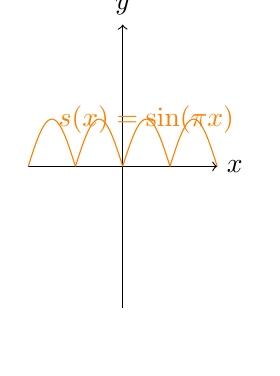
\begin{tikzpicture}[scale=0.6]
                \draw[->] (-2,0)--(2,0) node[right]{$x$};
                \draw[->] (0,-3)--(0,3) node[above]{$y$};
                % Unrolled loop for s(x)=sin(pi*x)
                \draw[domain=-2:-1,smooth,variable=\x,orange] plot({\x},{sin(3.14159*(\x+2) r)});
                \draw[domain=-1:0,smooth,variable=\x,orange] plot({\x},{sin(3.14159*(\x+1) r)});
                \draw[domain=0:1,smooth,variable=\x,orange] plot({\x},{sin(3.14159*\x r)});
                \draw[domain=1:2,smooth,variable=\x,orange] plot({\x},{sin(3.14159*(\x-1) r)});
                \node[orange,above] at (0.5,0.5) {$s(x)=\sin(\pi x)$};
            \end{tikzpicture}
        \end{tabular}
    \end{center}
    
    \begin{center}
        \begin{tabular}{cc} % 2x2 matrix structure
            % Top-left plot
            \begin{tikzpicture}[scale=0.6]
                \draw[->] (-2,0)--(2,0) node[right]{$x$};
                \draw[->] (0,-3)--(0,3) node[above]{$y$};
                % f(x) = |x|, even extension of f(x) = x
                \draw[domain=-1:1,smooth,variable=\x,blue] plot({\x},{abs(\x)});
                \draw[domain=1:2,smooth,variable=\x,blue] plot({\x},{abs(\x-2)});
                \draw[domain=-2:-1,smooth,variable=\x,blue] plot({\x},{abs(\x+2)});
                \node[blue,above right] at (0.5,0.5) {$f_{\text{even}}(x)=|x|$};
            \end{tikzpicture}
            &
            % Top-right plot
            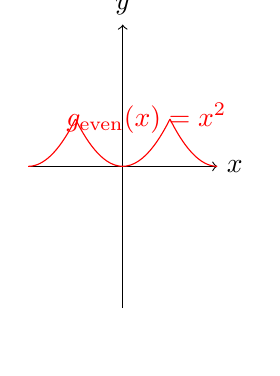
\begin{tikzpicture}[scale=0.6]
                \draw[->] (-2,0)--(2,0) node[right]{$x$};
                \draw[->] (0,-3)--(0,3) node[above]{$y$};
                % g(x) = x^2, even extension 
                \draw[domain=-1:1,smooth,variable=\x,red] plot({\x},{\x*\x});
                \draw[domain=1:2,smooth,variable=\x,red] plot({\x},{abs(\x-2)*abs(\x-2)});
                \draw[domain=-2:-1,smooth,variable=\x,red] plot({\x},{abs(\x+2)*abs(\x+2)});
                \node[red,above] at (0.5,0.5) {$g_{\text{even}}(x)=x^2$};
            \end{tikzpicture}
            \\
            % Bottom-left plot
            \begin{tikzpicture}[scale=0.6]
                \draw[->] (-2,0)--(2,0) node[right]{$x$};
                \draw[->] (0,-3)--(0,3) node[above]{$y$};
                % h(x) = e^|x|, even extension of h(x) = e^x
                \draw[domain=-1:1,smooth,variable=\x,green] plot({\x},{exp(abs(\x))});
                \draw[domain=1:2,smooth,variable=\x,green] plot({\x},{exp(abs(\x-2))});
                \draw[domain=-2:-1,smooth,variable=\x,green] plot({\x},{exp(abs(\x+2))});
                \node[green,above right] at (0.5,1.5) {$h_{\text{even}}(x)=e^{|x|}$};
            \end{tikzpicture}
            &
            % Bottom-right plot
            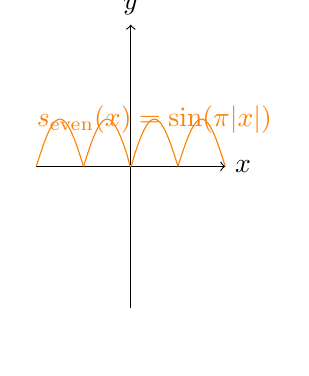
\begin{tikzpicture}[scale=0.6]
                \draw[->] (-2,0)--(2,0) node[right]{$x$};
                \draw[->] (0,-3)--(0,3) node[above]{$y$};
                % s(x) = sin(pi*|x|), even extension of s(x) = sin(pi*x)
                \draw[domain=-1:1,smooth,variable=\x,orange] plot({\x},{sin(3.14159*abs(\x) r)});
                \draw[domain=1:2,smooth,variable=\x,orange] plot({\x},{sin(3.14159*abs(\x-2) r)});
                \draw[domain=-2:-1,smooth,variable=\x,orange] plot({\x},{sin(3.14159*abs(\x+2) r)});
                \node[orange,above] at (0.5,0.5) {$s_{\text{even}}(x)=\sin(\pi|x|)$};
            \end{tikzpicture}
        \end{tabular}
    \end{center}

    \begin{center}
        \begin{tabular}{cc} % 2x2 matrix structure
            % Top-left plot
            \begin{tikzpicture}[scale=0.6]
                \draw[->] (-2,0)--(2,0) node[right]{$x$};
                \draw[->] (0,-3)--(0,3) node[above]{$y$};
                % f(x) = x, odd extension of f(x) = x
                \draw[domain=-1:1,smooth,variable=\x,blue] plot({\x},{\x});
                \draw[domain=1:2,smooth,variable=\x,blue] plot({\x},{\x-2});
                \draw[domain=-2:-1,smooth,variable=\x,blue] plot({\x},{\x+2});
                \node[blue,above right] at (0.5,0.5) {$f_{\text{odd}}(x)=x$};
            \end{tikzpicture}
            &
            % Top-right plot
            \begin{tikzpicture}[scale=0.6]
                \draw[->] (-2,0)--(2,0) node[right]{$x$};
                \draw[->] (0,-3)--(0,3) node[above]{$y$};
                % g(x) = x^2, odd extension
                \draw[domain=-2:-1,smooth,variable=\x,red] plot({\x}, {(\x+2)*(\x+2)});
                \draw[domain=-1: 0,smooth,variable=\x,red] plot({\x},-{\x*\x});
                \draw[domain= 0: 1,smooth,variable=\x,red] plot({\x}, {\x*\x});
                \draw[domain= 1: 2,smooth,variable=\x,red] plot({\x},-{(\x-2)*(\x-2)});
                \node[red,above] at (0.5,0.5) {$g_{\text{odd}}(x)$};
            \end{tikzpicture}
            \\
            % Bottom-left plot
            \begin{tikzpicture}[scale=0.6]
                \draw[->] (-2,0)--(2,0) node[right]{$x$};
                \draw[->] (0,-3)--(0,3) node[above]{$y$};
                % h(x) = e^x, odd extension
                \draw[domain=-2:-1,smooth,variable=\x,green] plot({\x}, {exp( \x+2)});
                \draw[domain=-1: 0,smooth,variable=\x,green] plot({\x},-{exp(-\x  )});
                \draw[domain= 0: 1,smooth,variable=\x,green] plot({\x}, {exp( \x  )});
                \draw[domain= 1: 2,smooth,variable=\x,green] plot({\x},-{exp(-\x+2)});
                \node[green,above right] at (0.5,1.5) {$h_{\text{odd}}(x)=e^x$};
            \end{tikzpicture}
            &
            % Bottom-right plot
            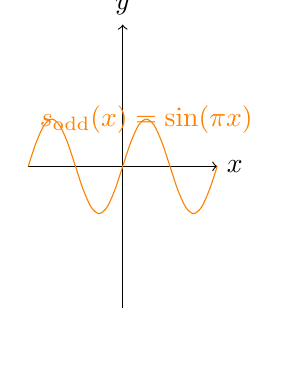
\begin{tikzpicture}[scale=0.6]
                \draw[->] (-2,0)--(2,0) node[right]{$x$};
                \draw[->] (0,-3)--(0,3) node[above]{$y$};
                % s(x) = sin(pi*x), odd extension
                \draw[domain=-2:2,smooth,variable=\x,orange] plot({\x},{sin(3.14159*\x r)});
                \node[orange,above] at (0.5,0.5) {$s_{\text{odd}}(x)=\sin(\pi x)$};
            \end{tikzpicture}
        \end{tabular}
    \end{center}
    We state the formulas for the even and odd extensions of period $2$.
    Over \([-1,1]\), define the even extensions:
    \begin{align*}
        f_{\text{even}}(x) &= |x|, 
        \\
        g_{\text{even}}(x) &= x^2,
        \\
        h_{\text{even}}(x) &= e^{|x|}, 
        \\
        s_{\text{even}}(x) &= |\sin(\pi x)|,
    \end{align*}
    and we define the odd extensions:
    \begin{align*}
        f_{\text{odd}}(x) &= x, 
        \\
        g_{\text{odd}}(x) &= \begin{cases}
        x^2 & x \in [0,1) \\
        -(-x)^2 = -x^2 & x \in [-1,0)
        \end{cases}
        \\
        h_{\text{odd}}(x) &= \begin{cases}
        e^x & x \in [0,1) \\
        -e^{-x} & x \in [-1,0)
        \end{cases}, 
        \\
        s_{\text{odd}}(x) &= \sin(\pi x).
    \end{align*}
\end{solution}



\begin{exercise}
    Consider the function 
    \begin{align*}
        f : [0,1] \to \bbR, \quad x \mapsto x^{3}.
    \end{align*}
    Extend this to an odd function with period $T = 2$. Sketch the graph of that function from $-2$ to $2$.
    Compute its Fourier coefficients in standard form. Compute the complex Fourier coefficients.
\end{exercise}
\begin{solution}
    We first sketch the odd extensions of that function:
    \begin{center}
    \begin{tikzpicture}[scale=0.6]
        \draw[->] (-2,0)--(2,0) node[right]{$x$};
        \draw[->] (0,-3)--(0,3) node[above]{$y$};
        % g(x) = x^2, odd extension
        \draw[domain=-2:-1,smooth,variable=\x,red] plot({\x}, {(\x+2)*(\x+2)*(\x+2)});
        \draw[domain=-1: 0,smooth,variable=\x,red] plot({\x}, {\x*\x*\x});
        \draw[domain= 0: 1,smooth,variable=\x,red] plot({\x}, {\x*\x*\x});
        \draw[domain= 1: 2,smooth,variable=\x,red] plot({\x},-{(\x-2)*(\x-2)*(\x-2)});
        \node[red,above] at (0.5,0.5) {$g_{\text{odd}}(x)$};
    \end{tikzpicture}
    \end{center}
    
\end{solution}







\begin{exercise}
    Suppose that
    \begin{align*}
        f(x) = \left\{\begin{array}{cc} x+1 & \text{ if $-1 < x < 0$ }, \\  1-x & \text{ if $ 0 < x < 1$ }, \\  0 & \text{ otherwise. } \end{array}\right.
        \qquad 
        g(x) = \left\{\begin{array}{cc} \frac 1 2 & \text{ if $-1 < x < 1$ }, \\ 0 & \text{ otherwise. } \end{array}\right.
        \qquad 
        h(x) = |x|
        .
    \end{align*}
    Compute the convolutions $u(x) = (f \star g)(x)$ and $v(x) = (g \star g)(x)$ and $w(x) = (g \star h)(x)$.
\end{exercise}
\begin{solution} 
\end{solution}



\begin{exercise}
    Suppose that $f(x) = x^2$ and that
    \begin{align*}
        g(x) = \left\{\begin{array}{cc} \frac 1 2 & \text{ if $-1 < x < 1$ }, \\ 0 & \text{ otherwise. } \end{array}\right.
        \qquad 
        h(x) = \left\{\begin{array}{cc} e^{-x} & \text{ if $x > 0$ }, \\ 0 & \text{ otherwise. } \end{array}\right.
    \end{align*}
    Compute the convolutions $u(x) = (f \star g)(x)$ and $v(x) = (f \star h)(x)$ .
\end{exercise}

\begin{solution}     
\end{solution}


\begin{exercise}
    We have discussed solutions to the differential equation 
    \begin{align*}
        - \Delta u(x) + k^2 u(x) = e^{-|x|}, \quad x \in \mathbb R.
    \end{align*}
    \begin{itemize}
        \item 
        Verify that, in the case $k=1$, we have a solution 
        \begin{align*}
            u(x) = \frac 1 2 (1+|x|) e^{-|x|} 
        \end{align*}
        Verify that every function of the form 
        \begin{align*}
            v(x) = \frac 1 2 (1+|x|) e^{-|x|} + c_1 e^{-x} + c_2 e^{x} 
        \end{align*}
        is a solution. For which values of $c_1$ and $c_2$ does the function decay towards zero as $x$ goes to $\pm \infty$?
        %
        \item 
        Verify that, in the case $k \neq 1$, we have a solution 
        \begin{align*}
            u(x) = - \frac{ e^{-k|x|} }{ 2k (k^2-1) } + \frac{ e^{-|x|} }{ k^2-1 }
        \end{align*}
        Verify that every function of the form 
        \begin{align*}
            v(x) = - \frac{ e^{-k|x|} }{ 2k (k^2-1) } + \frac{ e^{-|x|} }{ k^2-1 } + c_1 e^{-kx} + c_2 e^{kx} 
        \end{align*}        
        is a solution.
    \end{itemize}
\end{exercise}
\begin{solution}     
\end{solution}







\begin{exercise}
    We want to find a solution to the boundary value problem 
    \begin{gather*}
        - \Delta u(x) + k^2 u(x) = x, \quad 0 < x < L,
        \\
        u(0) = 0, \quad u(L) = 0.
    \end{gather*}
    \begin{itemize}
        \item Extend the right-hand side $f(x) = x$ to an odd function with period $2L$ and compute its Fourier coefficients.
        \item Using these coefficients, find the Fourier series of the solution $u$. Verify that the boundary condition $u(0) = u(L) = 0$ is satisfied.
    \end{itemize}
\end{exercise}
\begin{solution}     
\end{solution}




\begin{exercise}[Fun with Neumann boundary conditions]
    Consider the Poisson problem with \textit{Neumann boundary conditions} over the interval $[a,b] = [0,1]$: 
    \begin{gather*}
        - u''(x) + k^2 u(x) = x - \frac 1 2, \quad a < x < b,
        \\
        u'(a) = 0, \quad u'(b) = 0,
    \end{gather*}
    for some $k \geq 0$.
    \begin{enumerate}[label=(\alph*)]
        \item
        Extend $f(x) = x - \frac 1 2$ to an \textit{even} function over the real line with period $2$.
        \item 
        Compute the Fourier coefficients of that even extension of $f$.
        \item 
        Find the Fourier series of a function that satisfies the above differential equation.
    \end{enumerate}
\end{exercise}
\begin{solution}     
\end{solution}

\begin{exercise}[Fun with periodic boundary conditions]
    Consider the Poisson problem with \textit{periodic boundary conditions} over the interval $[a,b] = [0,1]$: 
    \begin{gather*}
        - u''(x) + k^2 u(x) = x - \frac 1 2, \quad a < x < b,
        \\
        u(a) = u(b),
    \end{gather*}
    for some $k \geq 0$.
    \begin{enumerate}[label=(\alph*)]
        \item
        Extend $f(x) = x - \frac 1 2$ to a $1$-periodic function over the real line.
        \item 
        Compute the Fourier coefficients of that extension of $f$.
        \item 
        Find the Fourier series of a function that satisfies the above differential equation.
    \end{enumerate}
\end{exercise}
\begin{solution}     
\end{solution}



% \begin{exercise}
% \end{exercise}
% \begin{solution}     
% \end{solution}
% 
% \begin{exercise}
% \end{exercise}
% \begin{solution}     
% \end{solution}

\end{document}

\begin{exercise}
    Find the Laplace transform $F(z)$ of 
    \begin{align*}
        f : \bbR_{0}^{+} \to \bbR, \quad t \mapsto t^{2}.
    \end{align*}
\end{exercise}
\begin{solution}     
    We compute 
    \begin{align*}
        F(z)&=\int_0^{\infty} t^2 e^{-z t} d t=\left[-\frac{t^2}{z} e^{-z t}\right]_0^{\infty}+\int_0^{\infty} \frac{2 t}{z} e^{-z t} d t \\ &=\left[\frac{2 t}{-z^2} e^{-z t}\right]_0^{\infty}+\int_0^{\infty} \frac{2}{z^2} e^{-z t} d t \\ &=\left[-\frac{2}{z^3} e^{-z t}\right]_0^{\infty} \\ &=0+\frac{2}{z^3} \\ &=\frac{2}{z^3}
        .
    \end{align*}
    Hence 
    \begin{align*}
        F(z)=\frac{2}{z^3} \quad \text { for } \mathrm{R}(z)>0.
    \end{align*}
\end{solution}

\begin{exercise}[Fun with Neumann boundary conditions 2]
    Suppose we have got a Poisson problem with Neumann boundary conditions over the interval $[a,b] = [0,1]$. 
    \begin{gather*}
        - u''(x) = f(x), \quad a < x < b,
        \\
        u'(a) = h_a, \quad u'(b) = h_b.
    \end{gather*}
    We need the compatibility condition 
    \begin{gather*}
        \int_a^b f(x) dx + ( h_b - h_a ) = 0.
    \end{gather*}
    \begin{enumerate}[label=(\alph*)]
        \item
        Find a constant function $c^f : [a,b] \to \bbR$ such that $f - c_f$ has integral zero.
        \item
        Use this to split up the original problem into two subproblems: 
        one with homogeneous boundary conditions, one with constant right-hand side, such that both problems satisfy the compatibility condition.
    \end{enumerate}
\end{exercise}
\begin{solution}     
\end{solution}



